
We apply our model to the smallholder farming communities on the western slope of Mount Kenya, specifically the Laikipia plateau, in east Africa as shown in Figure \ref{fig:map}. Laikipia county is located on the western (leeward) side of Mount Kenya and is adjacent to Meru and Nyeri counties in central Kenya. The county comprises smallholder agriculturalists, growing urban areas, and wildlife conservatories that attract tourism. The presence of dryland agriculturalists along a heterogeneous rainfall gradient makes the area suitable for an analysis of rainfall variability and cropping outcomes. The main cropping season for maize is planting around day 100 (first week of April) and harvesting around day 300 (last week of October) \cite{Ray2015}. % The study site receives on average 600-900 mm of rain per year and generally experiences two growing seasons around April and October \citep{Schmocker2016}.

Laikipia is a semiarid region prone to severe water deficits due to unreliable rainfall and high spatial and temporal variability. Rainfall in Kenya is characterized by a high coefficient of variability, which is common to semiarid environments \cite{herrero2010climate}. Furthermore, Laikipia has a heterogeneous landscape and complex topography that results in a rainfall gradient from 800-900 mm at the foothills of Mount Kenya to less than 500 mm in the northern end of the county \cite{wiesmann1998sustainable}. The annual distribution of rainfall is bimodal with two rainy seasons: the long (roughly March through May) and short (roughly October through December) rains. 

The Laikipia region of Kenya serves as an ideal study site to model the relationships between smallholder agriculture and climate variability for two reasons: (1) the tight couplings between food production and rainfall and (2) the prevalence of maize cultivation under various rainfall climatologies. In the region's drylands smallholder farmers face considerable challenges as rainfall arrives in pulses and in limited quantities for the majority of the year. Because the country has experienced a number of droughts in recent years, the Government of Kenya is especially interested in drought mitigation and increasing food security \cite{Kenya2010-jf}. Maize is an appropriate crop to study because it is grown under rainfed conditions and is an annual crop subject to both intermittent and terminal drought. Intermittent drought is caused by finite periods of inadequate water availability which does not necessarily result in crop failure whereas terminal drought is a progressive reduction in water availability that leads to crop failure before the end of the growing season \cite{neumann2008coping}.

\subsubsection{Soil Types}
We use the ISRIC Africa SoilGrids soil data base \cite{isric} to determine the soil textures found at depth 5-15 cm in our study site (Figure \ref{fig:map}). The region has a heterogeneous mix of soil textures. The most prevalent soil textures, at the points of the rainfall gauges, are clay, clay loam and sandy clay loam. Soils in our catchment are geologically young soils derived from basaltic volcanic rock and are generally fertile but susceptible to erosion. The clay soils have high water storage capacities, which can be suitable for growing maize \cite{muchena1988soils}. In Table \ref{soil} we show the corresponding values for the soil matrix potential at the hygroscopic point $\Psi_{s_{h}}$, and at field capacity $\Psi_{s_{fc}}$, the porosity $n$, and the saturated hydraulic conductivity $K_s$ according to the values found in \citeA{clapp1978empirical}.

\subsubsection{Historical Trends in Rainfall} \label{historic-rainfall}

We use long-term records of daily rainfall data for stations across the study site provided by the Centre for Training and Integrated Research in Arid and Semi-Arid Lands Development (CETRAD) in Nanyuki, Kenya. The gauges, shown in Figure \ref{fig:map}, have record lengths between 7 to 79 years. For computing statistics in Table \ref{table:mk}, we used stations with records of 40+ years. We considered temporal trends in the two parameters: $\alpha$, the average depth per rain event and $\lambda$, the average storm frequency per day during the two rainy seasons: long (March-May) and short (October-December) rains. To analyze inter-annual trends in the total seasonal rainfall and alpha and lambda parameters for the two seasons, we used a modified Mann-Kendall statistical test and the Theil-Sen estimator. Because the daily rainfall data is serially correlated, we use a variance corrected Mann-Kendall test proposed by \citeA{yue2004mann}, which detrends the serially correlated data and calculates an effective sample size using the lag-1 autocorrelation coefficient. We used the modified-mk package in R \cite{mmk}. 

\begin{figure}%[ht]
\centering
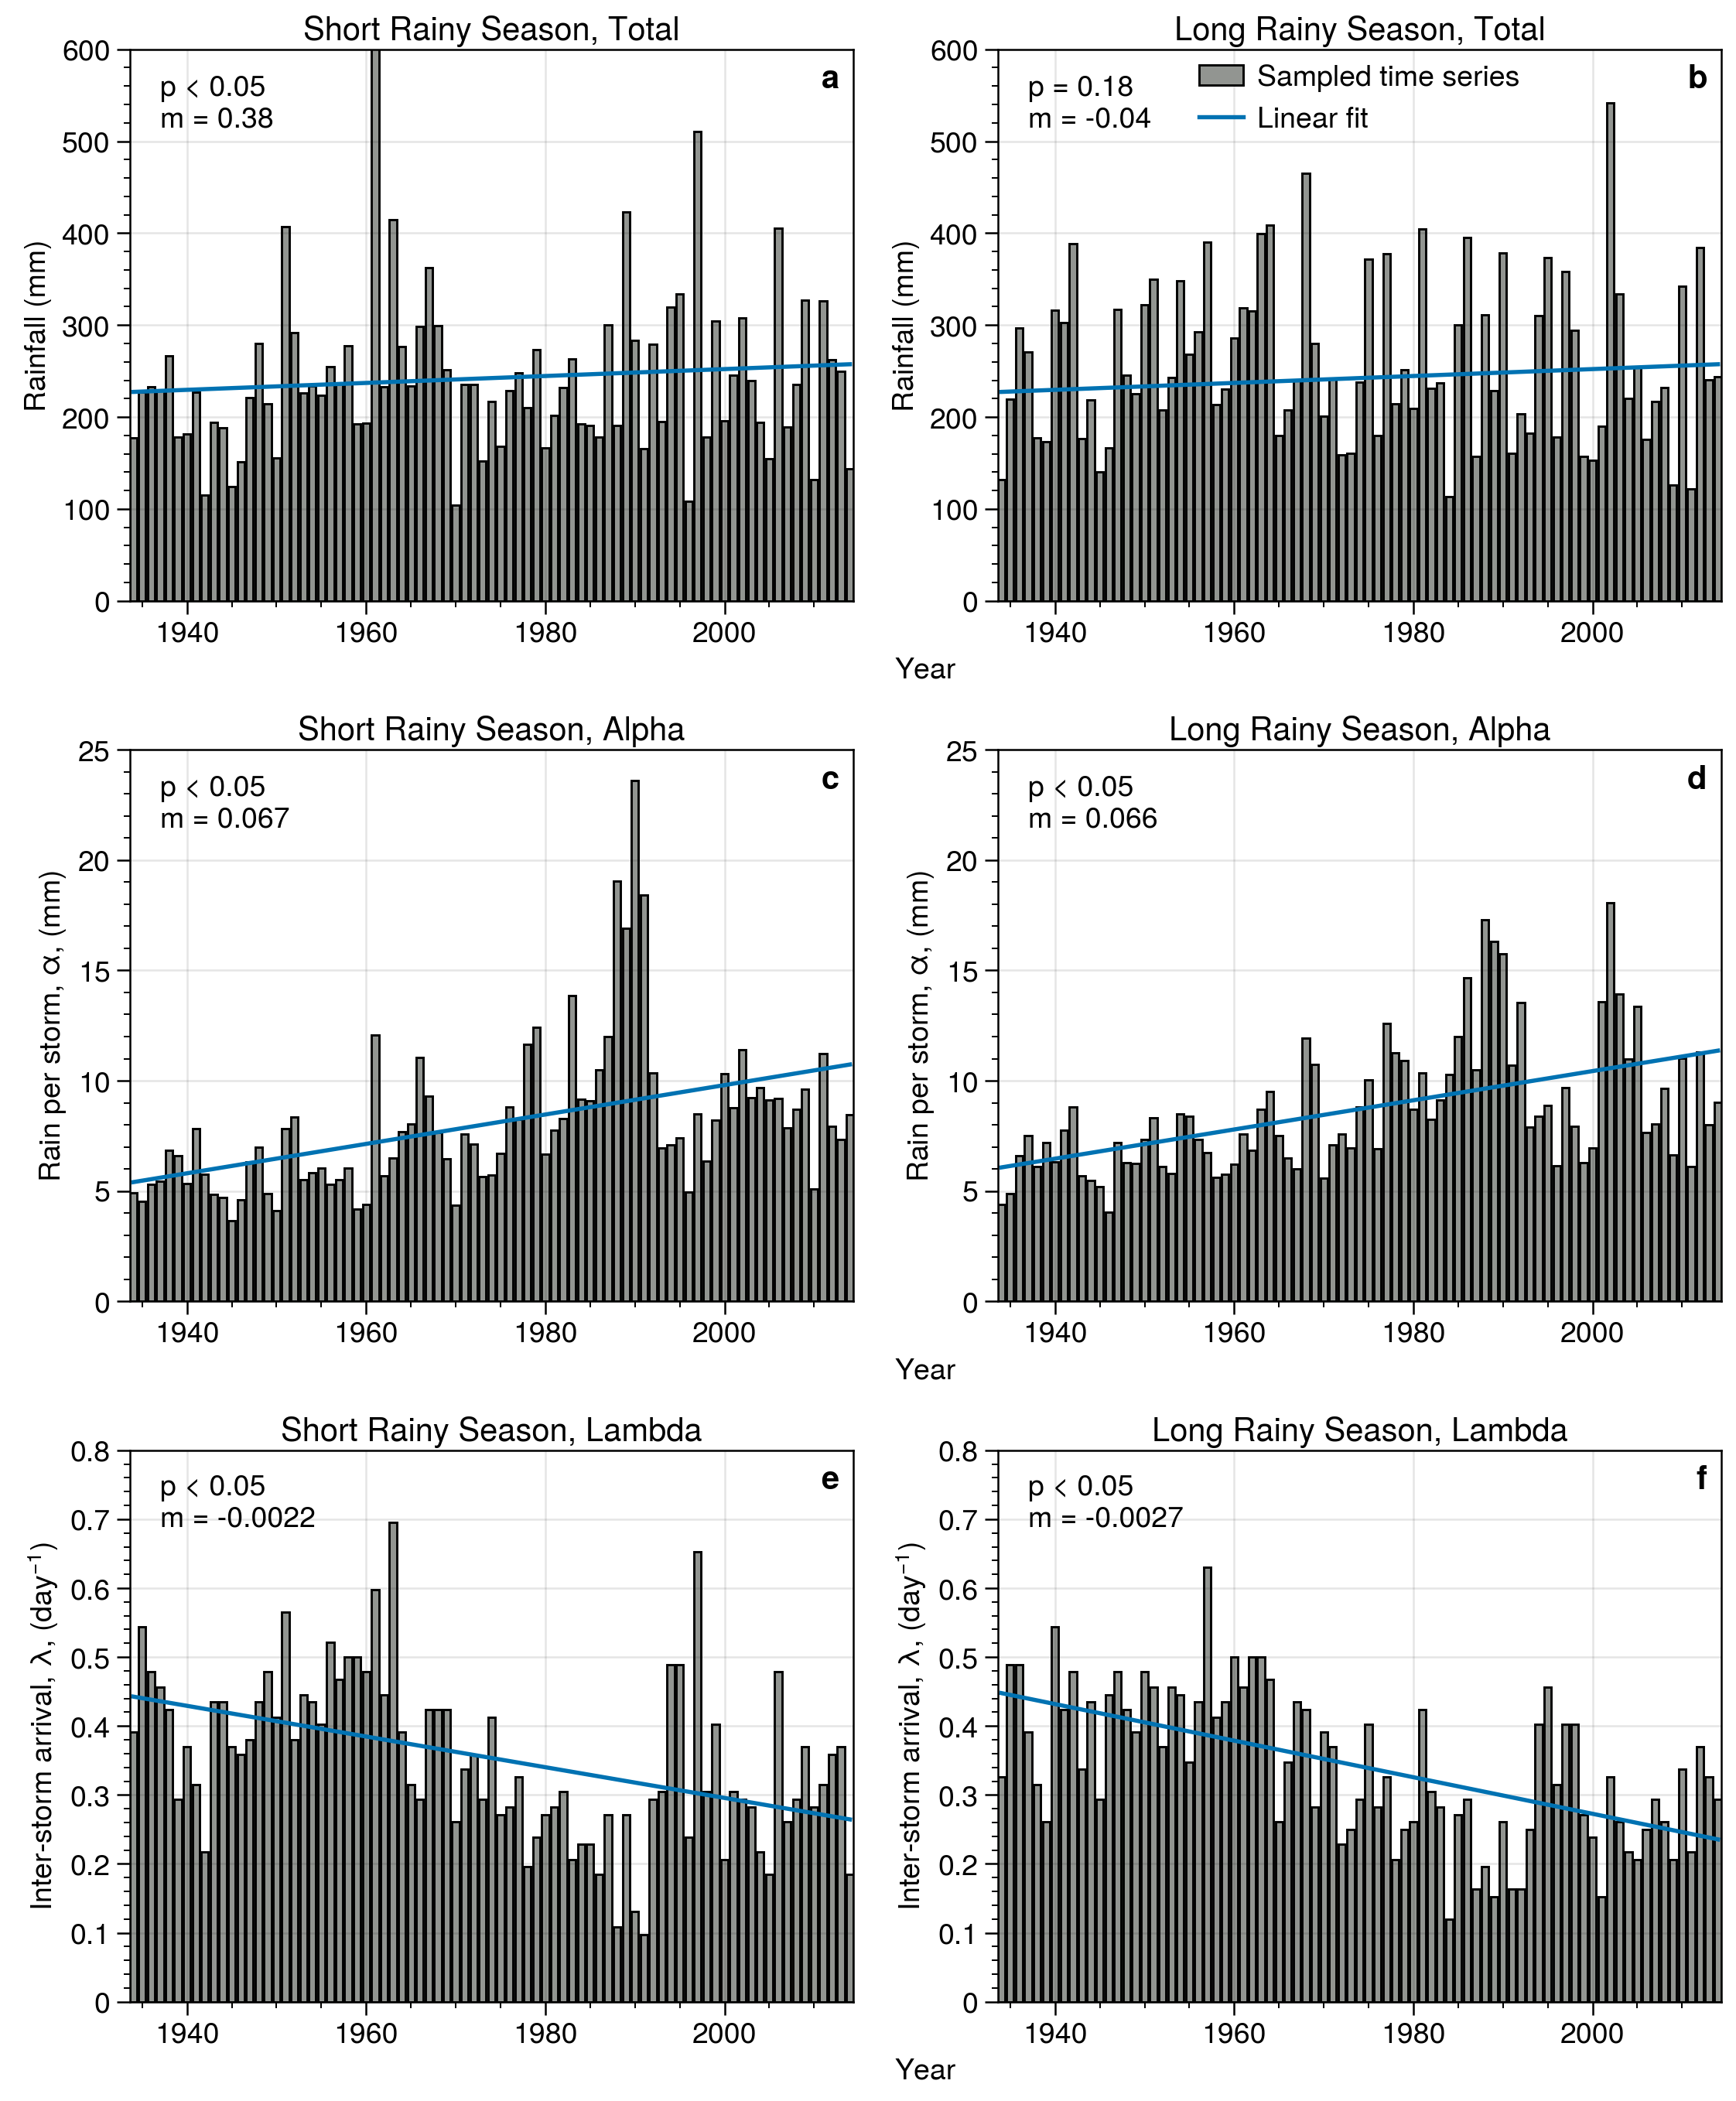
\includegraphics[width=155mm]{jacobson_ts.png}
\caption{Time series for the Jacobson Farm station which has a 79-year record length. Significant trends (p $<$0.05) are shown in plots a, c, d, e, f per the modified Mann-Kendall test.}
\label{fig:jacobson}
\end{figure}

\subsubsection{Maize Varieties and Yields}

In addition to being a function of environmental conditions and management decisions, total yields also depend on the maize variety. To define maximum potential yields for our simulations, we use empirical yield potentials for maize varieties typically grown by smallholder farmers in Laikipia. These data were sourced from Kenya Seed Company (see Figure \ref{fig:ksc}). We use the linear regression trend to set maximum potential yields for a range of maize varieties with maturity periods between 80 and 185 days. For each maize variety, we calculate a maximum potential yield, $Y_{max}$, which is used in Eq.~\ref{eq:yield}.

%Not actually including the text below, but could if we want to reduce max. yields again.
%Because potential yields are location-specific and the result of seed trials where water and nutrients are not limiting factors and biotic stress is controlled \cite{evans1993processes}, we altered the maximum yields to be more realistic with realized yields in Kenyan agriculture. Mention that this is different from actual yield (ya). We determined that a reasonable range of maize yields, irrespective of variety, is between 0.92 and 2.22 t/ha \cite{davenport2019using}. Therefore, we altered the minimum (1.28 t/ha) and maximum (5.04 t/ha) yield potentials from the seed companies based on the range in \cite{davenport2019using}, which led to a reduction of maximum values by 44\%. 

\begin{figure}%[ht]
\centering
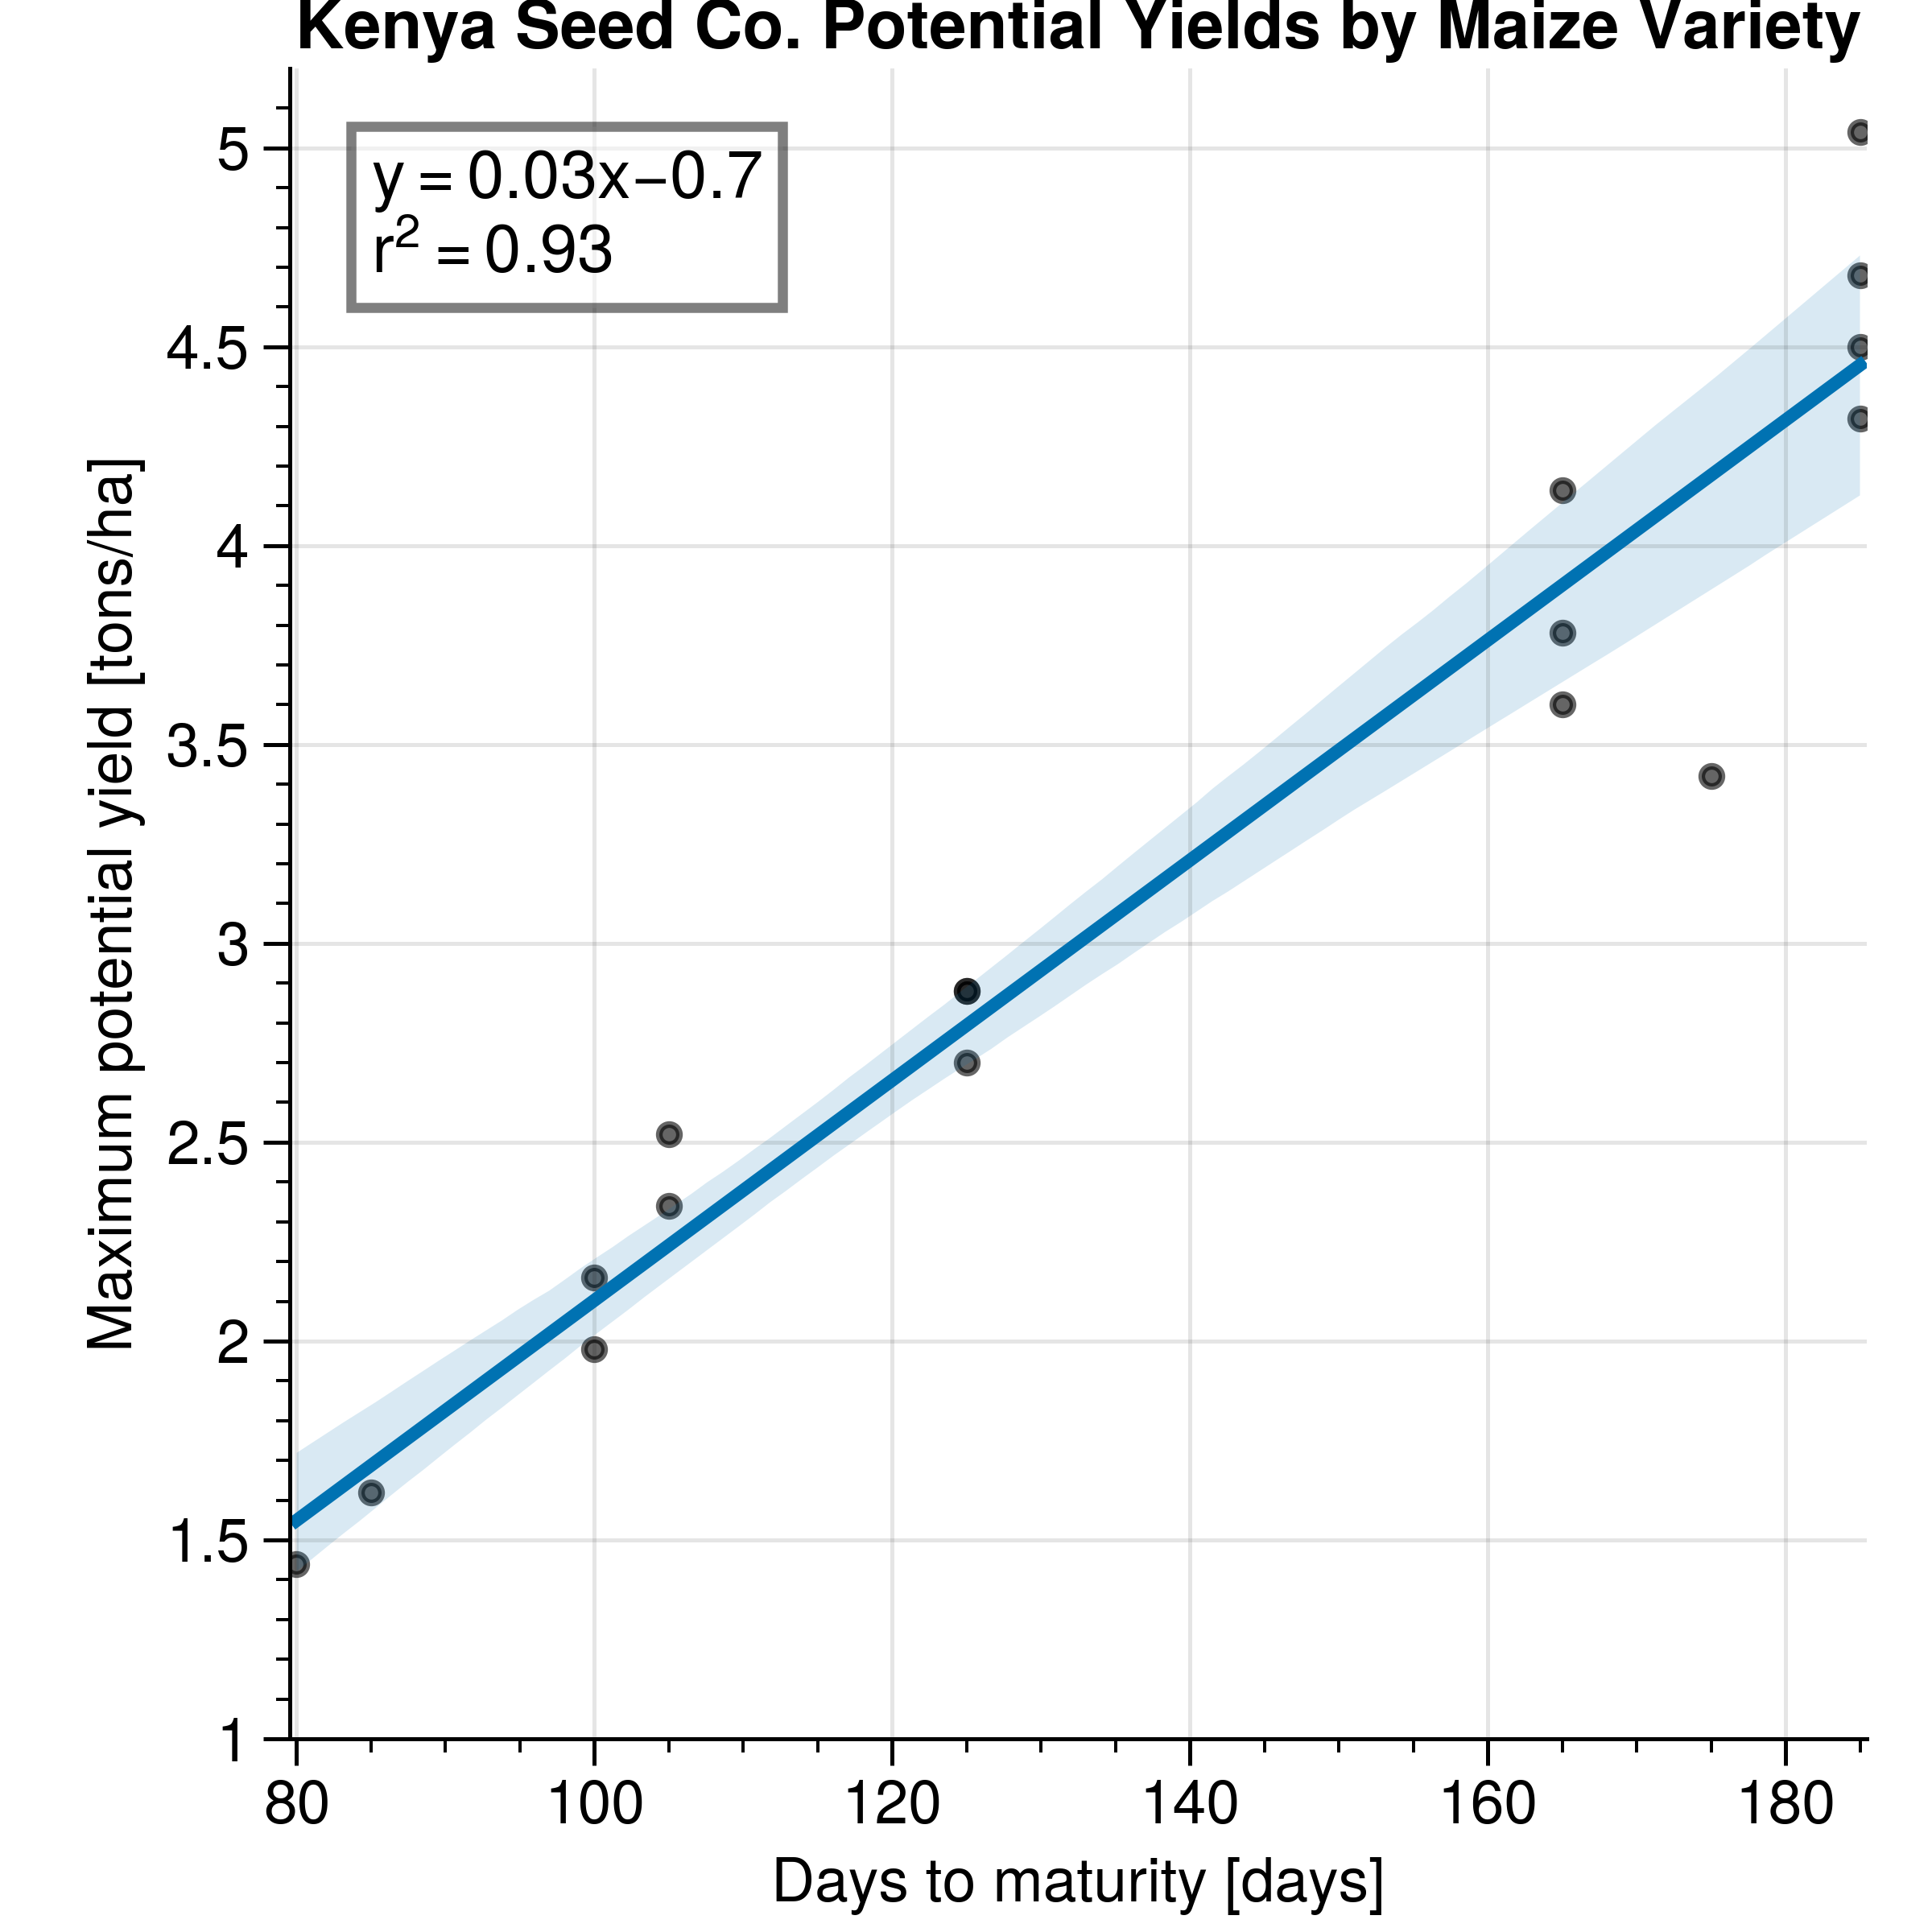
\includegraphics[width=80mm]{fig3_ksc.png}
\caption{Linear regression with 95\% confidence interval. Data are maize varieties sold by Kenya Seed Company. We removed two varieties from the dataset (PH1 and PH4) because the days to maturity information from Kenya Seed contradicted what is known about these four-month varieties. Data retrieved August 19 2019, from https://web.archive.org/web/20190216031348/http://kenyaseed.com/gallery/maize/.}

% Pretty sure that WRR is okay with having the citation in text as opposed to the reference list. If I do need it in the biblio use something like this: Highland maize varieties. (2019, February 16.) Kenya Seed Company Ltd. Retrieved August 19, 2019, from https://web.archive.org/web/20190216031348/http://kenyaseed.com/gallery/maize/. 

\label{fig:ksc}
\end{figure}

\begin{table}
\caption{Parameters associated with three prominent soil textures found within the study site.}
\centering
\begin{tabular}{l cccccc}
\hline
 Soil type  &  $\Psi_{s}$ (MPa)$^{b}$ & $b$$^{b}$ & $K_s$ (cm/d)$^{b}$ & $n$$^{b}$ & $s_h$ & $s_{fc}$ \\
\hline
  Clay & $-3.97 \times 10^{-3} $ &  11.4 & 11.1 & 0.482 & 0.503 & 0.830
  \\
  Clay loam  & $-6.17 \times 10^{-3}$  & 8.52 & 21.2 & 0.476 & 0.420 & 0.821 
  \\
  Sandy clay loam & $-2.93 \times 10^{-3}$ &  7.12 & 54.4 & 0.420 & 0.319 & 0.711
  \\
\hline
\multicolumn{7}{l}{$^{a}$We calculated values of $s_h$ and $s_{fc}$ assuming a soil water potential $\Psi_{h}=-10.0$ MPa} \\
\multicolumn{7}{l}{and $\Psi_{sfc} = -0.03$ MPa \cite{Laio2001-fe}.} \\
\multicolumn{7}{l}{$^{b}$\citeA{clapp1978empirical}.} \\
\end{tabular}
\label{soil}
\end{table}

%% SIDEWAYS FIGURE and TABLE
% AGU prefers the use of {sidewaystable} over {landscapetable} as it causes fewer problems.
%
 \begin{sidewaystable}
 \caption{Characteristics of rain gauges used in model simulations.$^{a}$}
\label{locations}
 \begin{tabular}{lcccccc}
\hline
Site &  Latitude &  Longitude &  Mean Annual Rainfall, mm & Altitude, m.a.s.l. & Start Year & End Year\\
\hline
Jacobson Farm & 0.04 & 37.04 & 735 & 1875 & 1934 & 2014 \\ %   0.040436,  37.043195
Ol Jogi Farm & 0.31 &  36.94 & 538 & 1741 & 1967 & 1999 \\ % Full lat, long 0.312581, 36.942360
\hline
\multicolumn{7}{l}{$^{a}$Start and end years are the years when the rainfall records began and ended for each rain gauge.}
 \end{tabular}
 \end{sidewaystable}

% \begin{table}
% \caption{Characteristics of rain gauges used in model simulations.}
% \begin{tabular}{lcccc}
% \hline
% Site &  Latitude &  Longitude &  Mean Annual Rainfall, mm & Altitude, m.a.s.l. \\
% \hline
% Jacobson Farm & 0.04 & 37.04 & 735 & 1875  \\ %   0.040436,  37.043195
% Ol Jogi Farm & 0.31 &  36.94 & 538 & 1741  \\ % Full lat, long 0.312581, 36.942360
% \hline
% \end{tabular}
% \label{locations}
% \end{table}
% % Could also put Record (years)